\documentclass[a4paper,10pt]{article}

\usepackage[utf8]{inputenc}
\usepackage[english]{babel}
%\usepackage[T1]{fontenc}
\usepackage{graphicx}
\usepackage{wrapfig}
\usepackage{amsmath, amssymb}
%\usepackage{listings}

\begin{document}

\author{Valentin Rosenberg, Zacharias Knudsen}
\date{\today}

\section{Clustering}

\subsection{1}
We will find clusters of a subset of our dataset, as the dataset is meant for regression, many attributes have little or no correlation. We want to examine if there are clusters in the following demographic, social and economic attributes:\\
racePctHisp, racePctWhite: The percentage of hispanics and whites in the community population respectively.\\
medIncome: The median income of the community.\\
NumStreet: The number of people living on the street.\\
NumImmig: The number of immigrants.\\
PctEmploy: The percentage of employed people.\\
PctPopUnderPov: The percentage under the poverty limit.\\
pctUrban: The percentage of people living in urban areas.\\

The data is fitted with a Gaussian Mixture Model and the AIC and BIC scores are calculated for each model as shown below. Each attribute is standardized and 200 objects are chosen for better runningtimes. 

\begin{figure}[h]
\centering
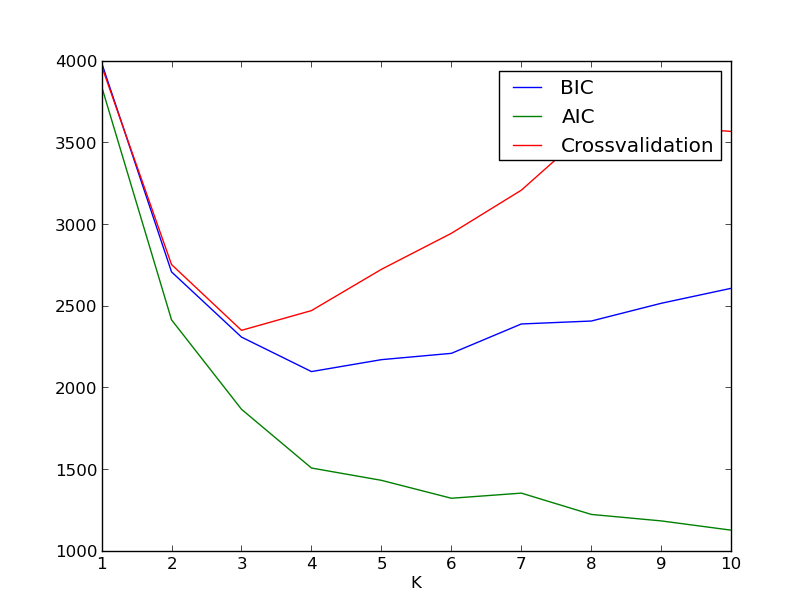
\includegraphics[h, width=0.8\textwidth]{figure_1}
\caption{10-fold crossvalidation, BIC and AIC for 1 to 10 clusters with a GMM. The vertical axis is the BIC, AIC and crossvalidation scores respectiveliy - crossvalidation is proportional to the negative log likelihood}
\end{figure}

The the crossvalidation score clearly has a minimum at 3 clusters, where BIC has a minimum at 4. AIC seems to not find its minimum at these numbers of clusters, maybe because of the high number of data objects. We chose 3 clusters as the cluster centres made the most sense.

The cluster centres are extracted and are as shown below.
\begin{verbatim}
['racePctHisp' 'racePctWhite' 'medIncome' 'NumStreet' 'NumImmig' 'PctEmploy'
 'PctPopUnderPov' 'pctUrban']
[[ 0.53793919 -0.73806562 -0.94107439 -0.05433901 -0.20753335 -0.94003235
   1.35819032 -1.02686909]
 [-0.4669858   0.58872669  0.39039555 -0.22532924 -0.27917154  0.14904979
  -0.49926193 -0.14320119]
 [ 0.51819432 -0.35295837 -0.00963756  0.77525982  0.51338927  0.19084485
  -0.09279508  0.68093829]]
\end{verbatim}
It seems the first cluster is one with many hispanics, low income, low employment, many living in poverty, and low urbanisation. The second cluster has a high number of whites, high income and few people under poverty limit. The third cluster is more interesting with many hispanics, normal income, high number of people on the street, high number of immigrants and high degree urbanization.

\subsection{2}
The data is also clustered with a hierarchical method, using euclidian distances as distance metric and a complete linkage function. The complete linkage function is chosen because we want well seperated clusters representing groupings in the communities. Also single linkage led to there being only one cluster, probably due to the chaining phenomenon.

\begin{figure}[h]
\centering
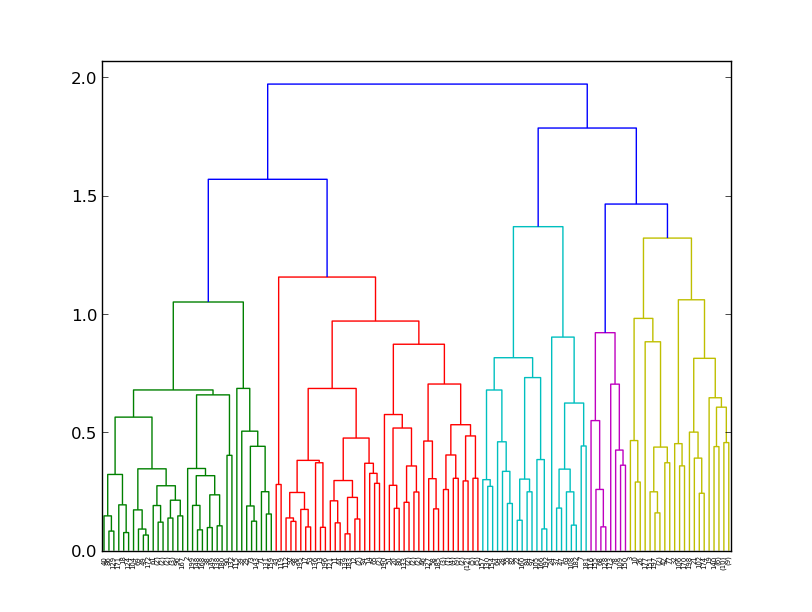
\includegraphics[h, width=0.8\textwidth]{figure_3}
\caption{Dendrogram of hierarchical clustering}
\end{figure}

\subsection{3}
We split the racePctWhite attribute into two classes deviding it by the median, as this might give a real separation of communities in these attributes given the history of America. If the clusters are grouped in this way, a confusion matrix will show a clear separation in the distribution of classes into the two categories.
\begin{figure}[h]
\centering
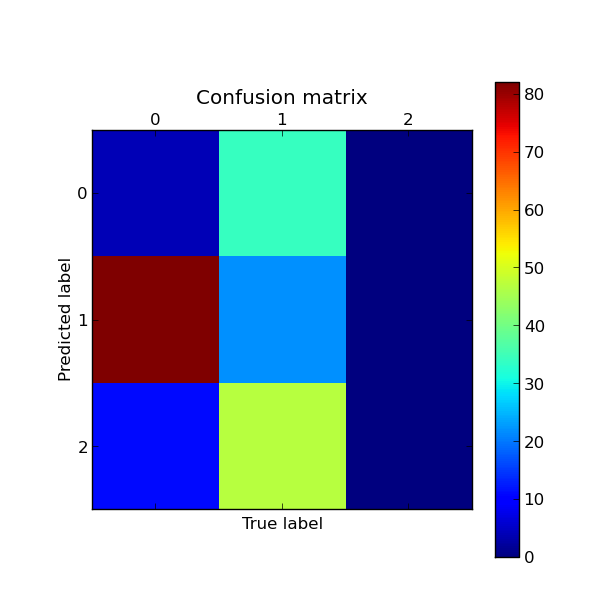
\includegraphics[h, width=0.8\textwidth]{figure_4}
\caption{Confusion matrix of true values of splitting racePctWhite and predicted clusters of the GMM.}
\end{figure}
As we can see the GMM has a clear separation of the two classes as the models cluster number 1 accounts for most of the low half of the racePctWhite attribute. The two other clusters 0 and 2 account for most of the upper half.

\begin{figure}[h]
\centering
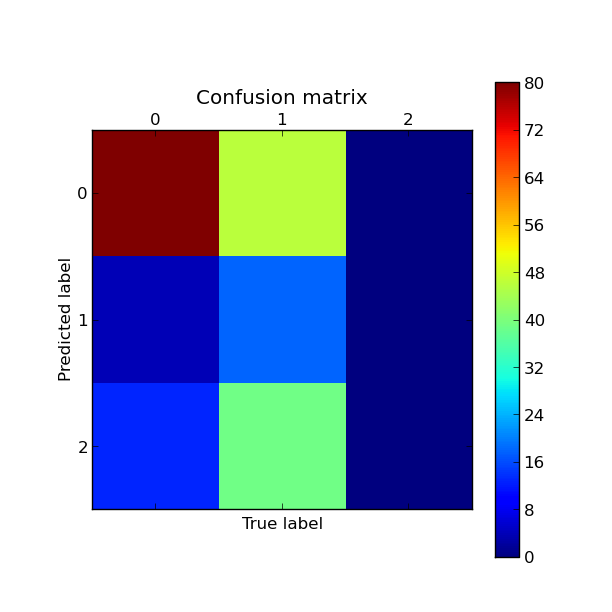
\includegraphics[h, width=0.8\textwidth]{figure_5}
\caption{Confusion matrix of true values of splitting racePctWhite and predicted clusters of the hierarchical clustering.}
\end{figure}
For the hierarchical clustering most of both the lower and upper half of racePctWhite are placed in the same cluster 0. Only some of the upper half is placed in cluster 2. The hierarchical clustering seems not to capture this given separation.


\end{document}
